% !TeX root = Bericht_main.tex
In der letzten Aufgabe, der wir uns im Rahmen dieser Berichte widmen wollen, wagen wir einen Blick über den (bisherigen) Tellerrand hinaus und werfen noch ein letztes Mal einen Blick auf das Regenwasserversickerungsmodell, von dem ausgehend wir uns bis hierher gearbeitet haben. Nun ist es aber so, dass wir bisher stets angenommen hatten, dass wir alle nötigen Informationen für unsere Verfahren, also sämtliche Randwerte sowie die Permeabilität $\kappa$ für jeden einzelnen Punkt des betrachteten Gebietes $D=(0,1)^2$ kennen.
Klar sollte jedoch sein, dass dies in der Realität eigentlich nie wirklich der Fall ist. Wir wollen deshalb im Folgenden auf eine Möglichkeit eingehen, mit dem Problem unsicherer Daten (am Beispiel einer unsicheren Permeabilität $\kappa$)  umzugehen.
\newline
Sei dazu $D \subset \R ^d$ das Rechengebiet und $(\Omega,\mathcal{A} ,\mathbb{P})$. Dabei ist $\mathbb{P} (A)$ die Wahrscheinlichkeit für ein Ereignis $A \in \mathcal{A}$ und $\mathbb{P} (\Omega ) = 1$.
\newline
Zu $x \in D$ ist dann	$\kappa (\cdot ,x ) : \Omega \rightarrow [\kappa_0,\kappa_1] $ die (vom Zufall abhängige) Permeabilität.
Wir betrachten also das folgende Randwertproblem:
\begin{gather*}
	\begin{cases}
	- \dive( \kappa(\omega,x)\nabla u(\omega,x))=0 &\text{, für } x \in D \\
	q(\omega , x) = - \kappa(\omega ,x) \nabla u &\text{, für }  x \in D\\
	-q(\omega,x) \cdot n = g_N &\text{, für } x \in \GammaN\\
	u(\omega,x) = u_D(\omega,x) &\text{, für } x \in \GammaD. 
	\end{cases}
\end{gather*}
Dabei stellen wir uns die Aufgabe den 'Erwartungswert' eines gegebenen Zielfunktionals $Q$, z.B. $Q(q) = \int_{\Gamma} q \cdot n \diff x $ (den Ausfluss) zu bestimmen.
Für die Verteilung von $\kappa (\omega,x )$ kommen zunächst viele verschiedene Verteilungen in Frage, doch nicht bei allen konvergiert ein Monte-Carlo-Verfahren (näheres dazu gleich), weswegen wir als (funktionierenden) Ansatz $\kappa (\omega,x )$  als log-normal-verteiltes stochastisches Feld mit Kovarianzfunktion $C(x,y)= \sigma^2 \exp ( - \norm{x-y}^{\alpha}_2 / \lambda^{\alpha})$ wählen. \\
Als Zielfunktional wählen wir das $L^2$-Funktional der Lösung $u(\omega,\cdot)$ des oben beschriebenen Randwertproblems, welches wir ab jetzt mit $Q$ bezeichnen wollen.
Da wir die konkreten Daten von $\kappa$ nicht kennen, sind wir an einem Schätzer für $\mathbb{E}[Q]$ interessiert.
Beachte hierbei, dass wir auch $u$ (die klassische Lösung des obigen Problems) nicht kennen, aber wir können $u$ mit der FEM approximieren. \\
Wir betrachten dazu zunächst folgenden Monte-Carlo Ansatz:
\begin{align*}
	    \hat{Q}^{MC}_{h,M}  \coloneqq \frac{1}{M} \sum_{i= 1}^{M} Q_h (\omega_i)
\end{align*}
Wir erhalten dabei als Fehler (RMSE - root mean square error):
\begin{align*}
	e(\hat{Q}^{MC}_{h,M})^2 = \mathbb{E} \bigl[ (\hat{Q}^{MC}_{h,M} - \mathbb{E}[Q] )^2\bigr] = M^{-1} \mathbb{V}[ Q_h] + (\mathbb{E}[Q_h -Q])^2
\end{align*}
Problematisch bei diesem Ansatz sind allerdings die (Rechen-)Kosten, der Ansatz ist schlichtweg nicht effizient genug. Um vernünftige Ergebnisse zu erhalten brauchen wir mindestens einige hundert 'Testsamples', wir haben aber gesehen, das schon die Berechnung eines solchen Samples auf einem mittleren bis hohen Level, auf einem 'normalen' Rechner durchaus einige Zeit in Anspruch nehmen kann. Stellen wir uns jetzt vor wir müssten für jede Rechnung mehr als das hundertfache an Zeit einplanen sehen wir schnell ein, dass dieser Ansatz maximal für sehr einfache kleine Probleme zielführend ist.
Dieses Problem führt uns schließlich auf die Multilevel Monte Carlo Methode (MLMC). \\
Hauptidee hierbei ist die beiden Konzepte der Monte Carlo Methode und der bereits zu einem früheren Zeitpunkt der Vorlesung eingeführten Multilevel-Verfahren zu vereinigen und so eine Balance zwischen Kosten der einzelnen Samples und Gesamtkosten herzustellen.
So wird versucht auf dem höchsten Level so wenig Samples wie nötig zu berechnen und dafür viele Samples auf den kostengünstigeren niedrigeren Leveln durchzuführen und möglichst trotzdem die Genauigkeit des höheren Levels zu erhalten.

Wir stellen also den MLMC-Schätzer auf:
\begin{align*}
     \hat{Q}^{MLMC}_{h,\{ M_l \}_{l=0}^{L}} = \sum_{l = 0}^{L} \hat{Y}_{h,M_l}^{MC} = \sum_{l=0}^{L} \frac{1}{M_l} \sum_{i=1}^{M_l} Y_l(w_i)
\end{align*} 
wobei $Y_0(\omega) = Q_0(\omega)$ und $Y_l(\omega) = Q_l(\omega) - Q_{l-1}(\omega)$ \\
\underline{Beobachtung:}
\begin{align*}
	&\underbrace{\mathbb{E}[\hat{Q}^{MC}_{h_L}]} = \mathbb{E}[Q_{h_0}]+ \sum_{l=1}^{L} \mathbb{E}[Q_{h_l}-Q_{h_{l-1}}] = \sum_{l=0}^{L} \mathbb{E}[\hat{Y}_l]\\
	&\text{MC-Schätzer auf höchstem Level}
\end{align*}
Als Fehler erhalten wir dabei:
\begin{align*}
	e(\hat{Q}^{MLMC}_{h,\{ M_l \}_{l=0}^{L}})^2 = \mathbb{E} \bigl[ (\hat{Q}^{MLMC}_{h,\{ M_l \}_{l=0}^{L}} - \mathbb{E}[Q] )^2\bigr] =\underset{\text{Fehler des Schätzers}}{\underbrace{\sum_{l=0}^{L} \frac{1}{M_l} \mathbb{V}[Y_l] }} + \underset{\text{FEM Fehler}}{\underbrace{(\mathbb{E}[Q_h-Q])^2}}
\end{align*}
Damit die Methode konvergiert sind die folgenden Voraussetzungen zu überprüfen: 
\begin{enumerate}
	  \item Die Konvergenzrate $\alpha$ der FEM ist gegeben durch
		  \begin{align*}
		       |\mathbb{E}[Q_h-Q]| \lesssim h^{\alpha} \qquad |\mathbb{E}[Q_h-Q]| \lesssim N^{- \alpha} \qquad
		       \text{wobei N = dim} (V_h) 
		  \end{align*}
	\item Die Kosten der FEM können abgeschätzt werden durch 
		\begin{align*}
		    C(Q_h) \lesssim h^{-\gamma}  \qquad 
		    C(Q_h) \lesssim N^{\gamma}
		\end{align*}
	\item Die Varianz der Differenz $Q_{h_l} - Q_{h_{l-1}}$ fällt mit 
		\begin{align*}
			|\mathbb{V}[Q_{h_l}-Q_{h_{l-1}}]| \lesssim h^{\beta} \qquad 
			|\mathbb{V}[Q_{h_l}-Q_{h_{l-1}}]| \lesssim N^{- \beta} \qquad
		\end{align*}
\end{enumerate}
Dazu testen wir obige Bedingungen zunächst mit verschiedenen Parametern der verwendeten Covarianzfunktion $C(x,y)= \sigma^2 \exp ( - \norm{x-y}^{\alpha}_2 / \lambda^{\alpha})$
\begin{figure}[H]
	\centering
	\captionabove{Konvergenztest für verschieden Parameter}
	\subfigure[$\sigma = 1 \qquad \lambda =0.15 \qquad \alpha= 1,8$]{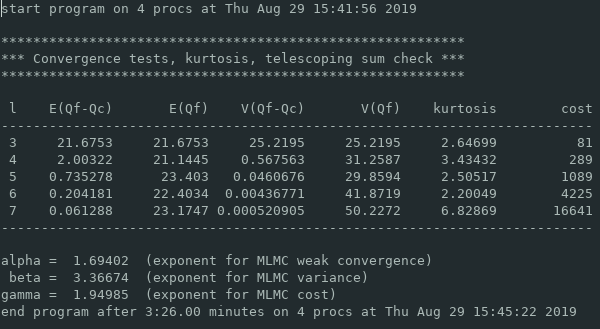
\includegraphics[width=0.45\textwidth]{../Aufgabe39/Sigma1/par.png}}	 
	\subfigure[$\sigma = 3 \qquad \lambda =0.15 \qquad \alpha= 1,8$]{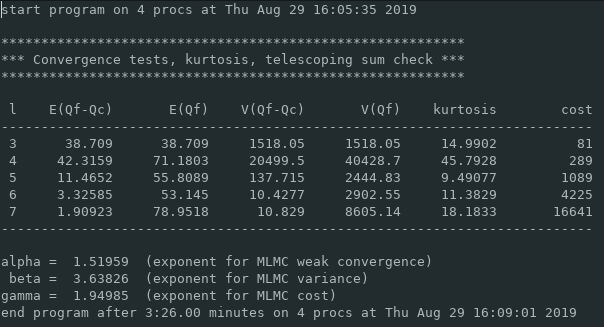
\includegraphics[width=0.45\textwidth]{../Aufgabe39/Sigma3/par.png}}	
	\subfigure[$\sigma = 1 \qquad \lambda =0.15 \qquad \alpha= 0.9$]{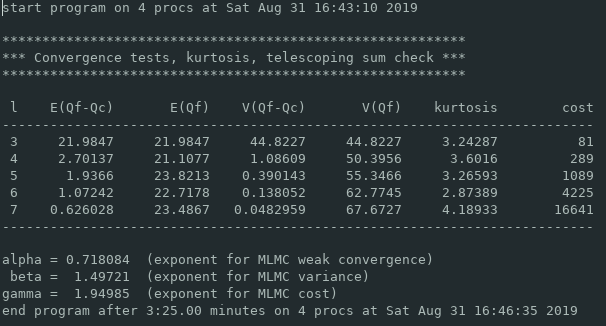
\includegraphics[width=0.45\textwidth]{../Aufgabe39/Sigma1alpha0.9/par.png}}	
	\subfigure[$\sigma = 1 \qquad \lambda =0.05 \qquad \alpha= 1.8$]{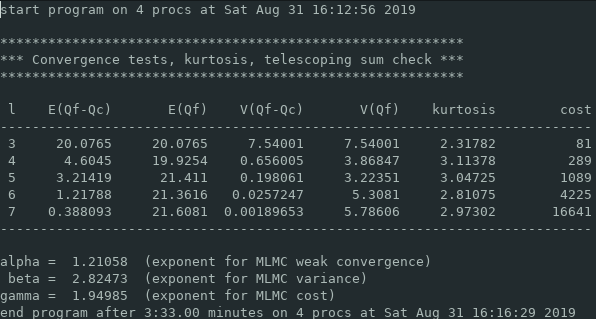
\includegraphics[width=0.45\textwidth]{../Aufgabe39/Sigma1lamda0.05/par.png}}	
\end{figure}

Zudem können wir Beispiele der entstandenen Permeabilitäten einzelner Samples betrachten um ein Gefühl dafür zu bekommen, wie die unterschiedlichen Parameter das stochastische Feld beeinflussen:

\begin{figure}[H]
	\centering
	\captionabove{Beispielpermeabilitäten für verschiedene $\sigma$ unter derselben Skalierung}
	\subfigure[$\sigma = 1 \; \lambda =0.15  \; \alpha= 1.8$]{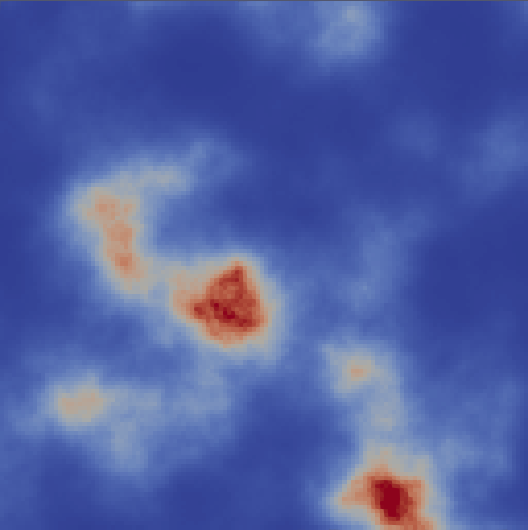
\includegraphics[width=0.25\textwidth]{../Aufgabe39/Sigma1/perm2.png}}	 
	\subfigure[$\sigma = 3  \; \lambda =0.15 \; \alpha= 1.8$]{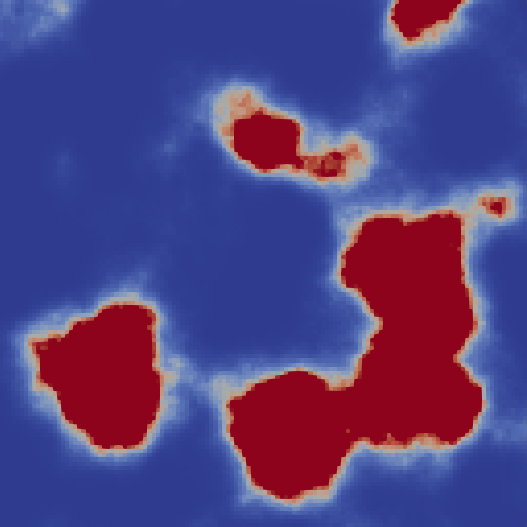
\includegraphics[width=0.25\textwidth]{../Aufgabe39/Sigma3/perm2.png}}	
	\subfigure[$\sigma = 6  \; \lambda =0.15  \; \alpha= 1.8$]{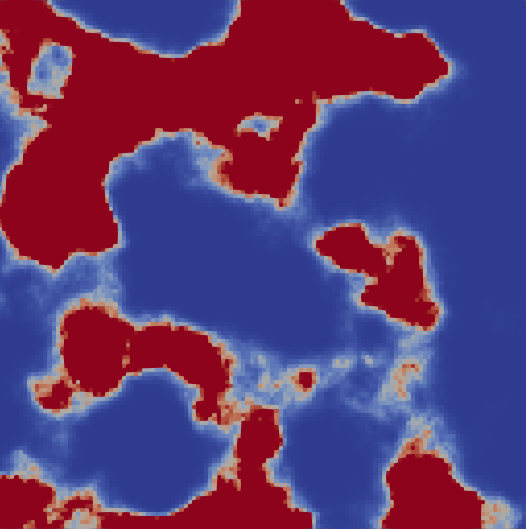
\includegraphics[width=0.25\textwidth]{../Aufgabe39/Sigma6/perm2.png}}	
\end{figure}
$\sigma$ geht in die Varianz der einzelnen Zufallsvariablen ein. An den Permeabilitäten erkennt man das daran, dass der Bereich $[\sigma_0,\sigma_1] $ immer größer wird und wir bei größerem Sigma (wenn wir über die gleichen Werte skalieren) deutlich mehr Bereiche auf oder jenseits des ursprünglichen Maximalniveaus finden.
\begin{figure}[H]
	\centering
	\captionabove{Beispielpermeabilitäten für verschiedene $\lambda$ unter derselben Skalierung}
	\subfigure[$\sigma = 1 \; \lambda =0.05  \; \alpha= 1,8$]{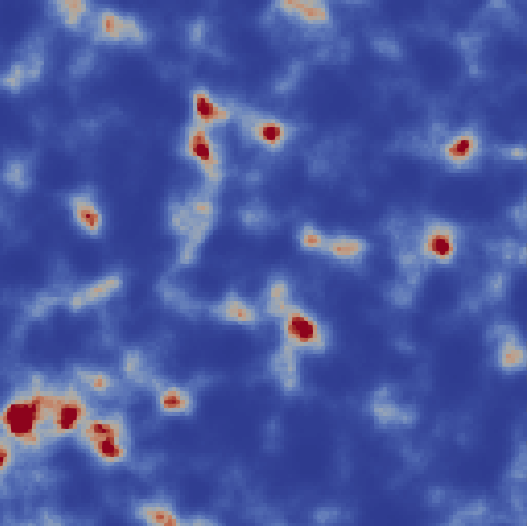
\includegraphics[width=0.25\textwidth]{../Aufgabe39/Sigma1lamda0.05/perm2.png}}	 
	\subfigure[$\sigma = 1  \; \lambda =0.15 \; \alpha= 1.8$]{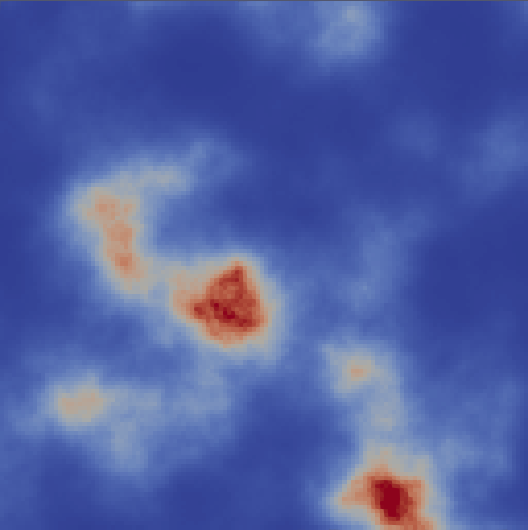
\includegraphics[width=0.25\textwidth]{../Aufgabe39/Sigma1/perm2.png}}	
	\subfigure[$\sigma = 1  \; \lambda =0.27  \; \alpha= 1.8$]{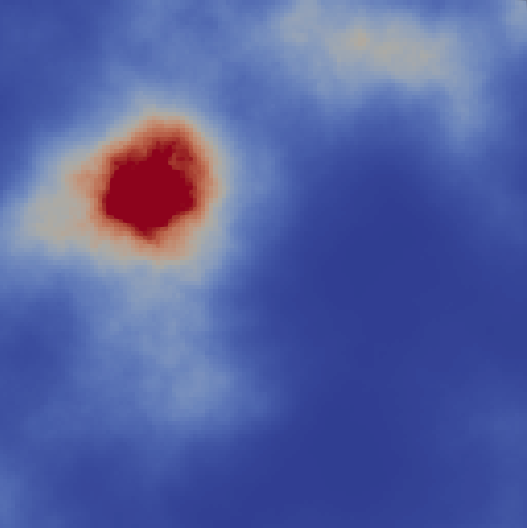
\includegraphics[width=0.25\textwidth]{../Aufgabe39/Sigma1lamda0.27/perm2.png}}	
\end{figure}
Mit $\lambda$ können wir die Korrelationslänge steuern, so erhalten wir für ein großes $\lambda$ größere zusammenhängende Bereiche während sich bei sehr kleinem $\lambda$ viele kleinere Bereiche bilden, da einzelne Punkte nur im Bereich der jetzt geringeren Korrelationslänge miteinander korrelieren.

\begin{figure}[H]
	\centering
	\captionabove{Beispielpermeabilitäten für verschiedene $\alpha$ unter derselben Skalierung}
	\subfigure[$\sigma = 1 \; \lambda =0.15  \; \alpha=0.9$]{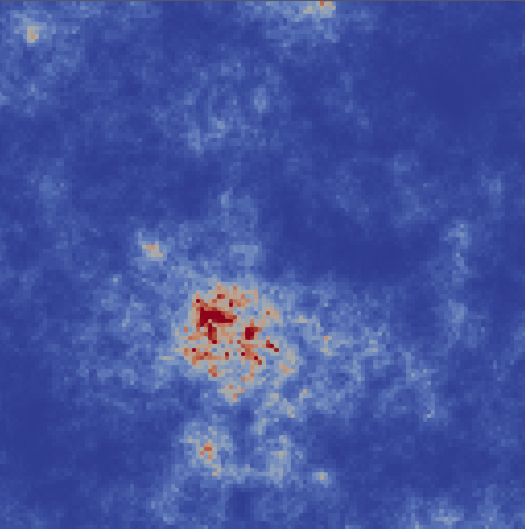
\includegraphics[width=0.25\textwidth]{../Aufgabe39/Sigma1alpha0.9/perm2.png}}	 
	\subfigure[$\sigma = 1  \; \lambda =0.15 \; \alpha= 1.8$]{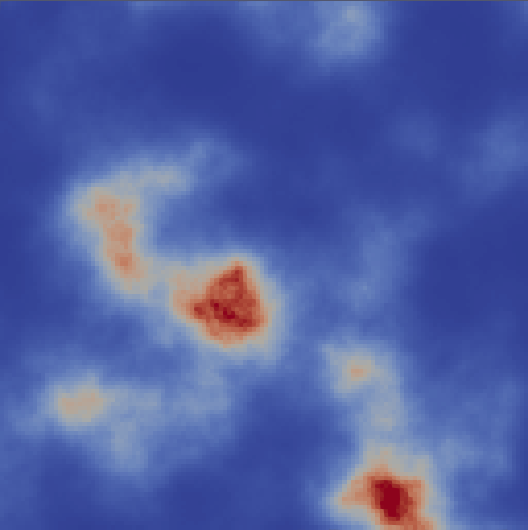
\includegraphics[width=0.25\textwidth]{../Aufgabe39/Sigma1/perm2.png}}	
	\subfigure[$\sigma = 1  \; \lambda =0.15  \; \alpha=  2.7$]{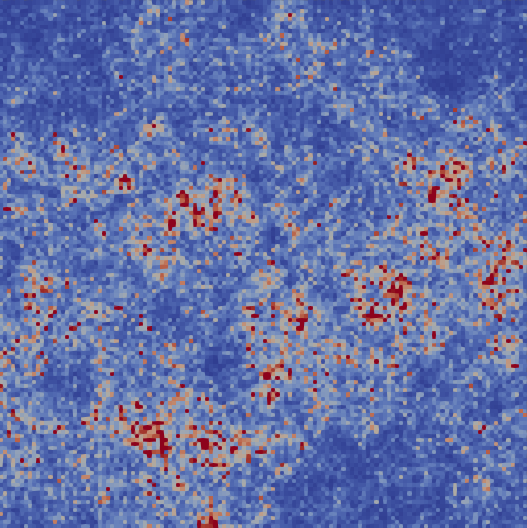
\includegraphics[width=0.25\textwidth]{../Aufgabe39/Sigma1alpha2.7/perm2.png}}	
\end{figure}
Mit $\alpha$ können wir die 'Art' der Korrelation ändern, besonders gut sieht man das beim Vergleich der Permeabilitäten von $\alpha = 1,8$ und $\alpha = 2.7$. Während wir für letzteres ein stark unkorreliertes Bild erhalten sind die Strukturen für $\alpha = 1.8$ innerhalb des Korrelationsbereiches (also jeweils für $| x-y|$ kleiner gleich der Korrelationslänge) schön korreliert und daher glatt. \\
Je nach Parameterwahl erhalten wir so mal mehr mal weniger gute Konvergenzeigenschaften des Verfahrens. Dies spiegelt sich zum einen in den Konvergenzgrößen $\alpha$, $ \beta$, $\gamma$ (Vorsicht: dies ist  nicht das $\alpha$ aus der Kovarianzfunktion), zum anderen aber auch an den Konvergenzplots der Größen $\mathbb{E}[Q_{h_l}]$,  $\mathbb{E}[Q_{h_l} - Q_{h_{l-1}}]$, $\mathbb{V}[Q_{h_l}]$,  $\mathbb{V}[Q_{h_l} - Q_{h_{l-1}}]$.
\begin{enumerate}
	\item $\sigma = 1$, $\lambda = 0.15$, $\alpha= 1.8$ $\Rightarrow$ $\alpha = 1.69$, $\beta = 3.37$, $\gamma = 1.95$
	\item $\sigma = 6$, $\lambda = 0.15$, $\alpha= 1.8$ $\Rightarrow$ $\alpha = 1.32$, $\beta = 2.88$, $\gamma = 1.95$
	\item $\sigma = 1$, $\lambda = 0.05$, $\alpha= 1.8$ $\Rightarrow$ $\alpha = 1.21$, $\beta = 2.82$, $\gamma = 1.95$
	\item $\sigma = 1$, $\lambda = 0.15$, $\alpha= 2.7$ $\Rightarrow$ $\alpha = 0.14$, $\beta = 0.39$, $\gamma = 1.95$
\end{enumerate}

\begin{figure}[H]
	\centering
	\captionabove{Zugehörige Kovergenzplots zu den oben angeführten Beispielkonfigurationen}
	\subfigure[1.]{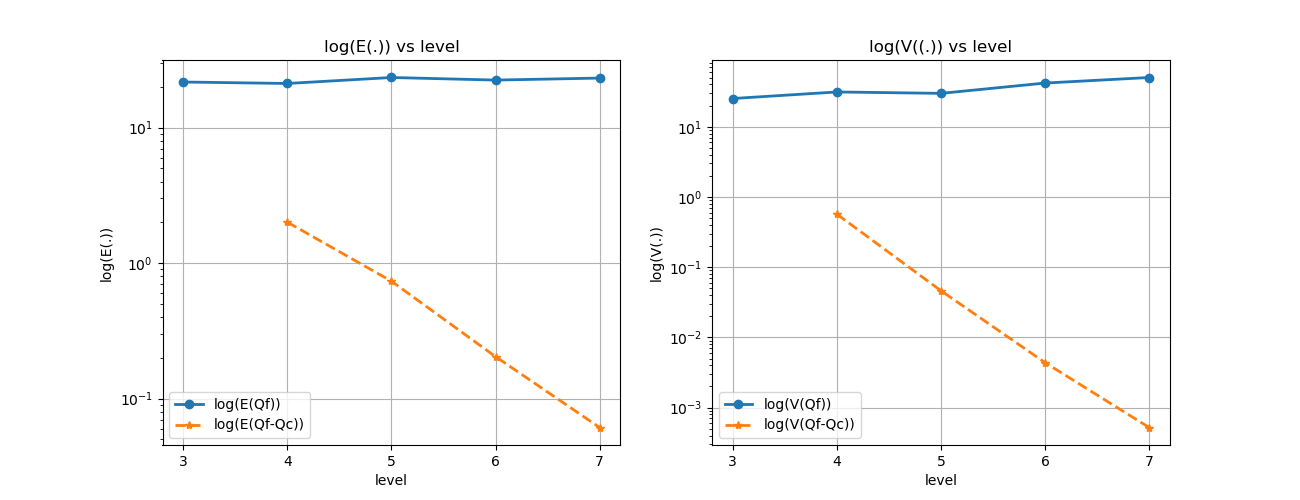
\includegraphics[width=0.49\textwidth]{../Aufgabe39/Sigma1/plotmc_sigma1.png}}	 
	\subfigure[2.]{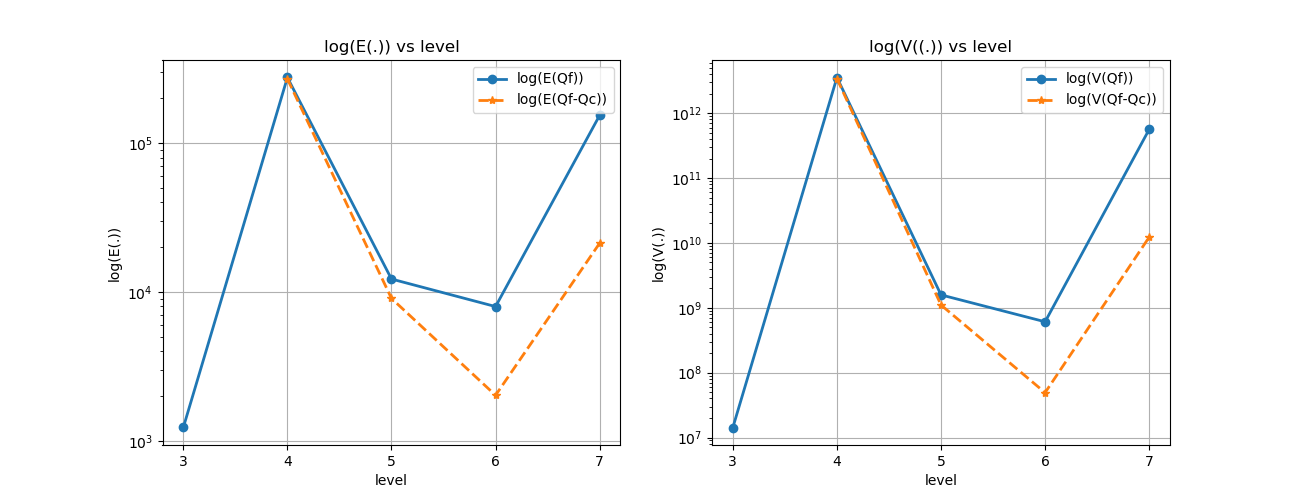
\includegraphics[width=0.49\textwidth]{../Aufgabe39/Sigma6/plot_mcsig6.png}}	
	\subfigure[3.]{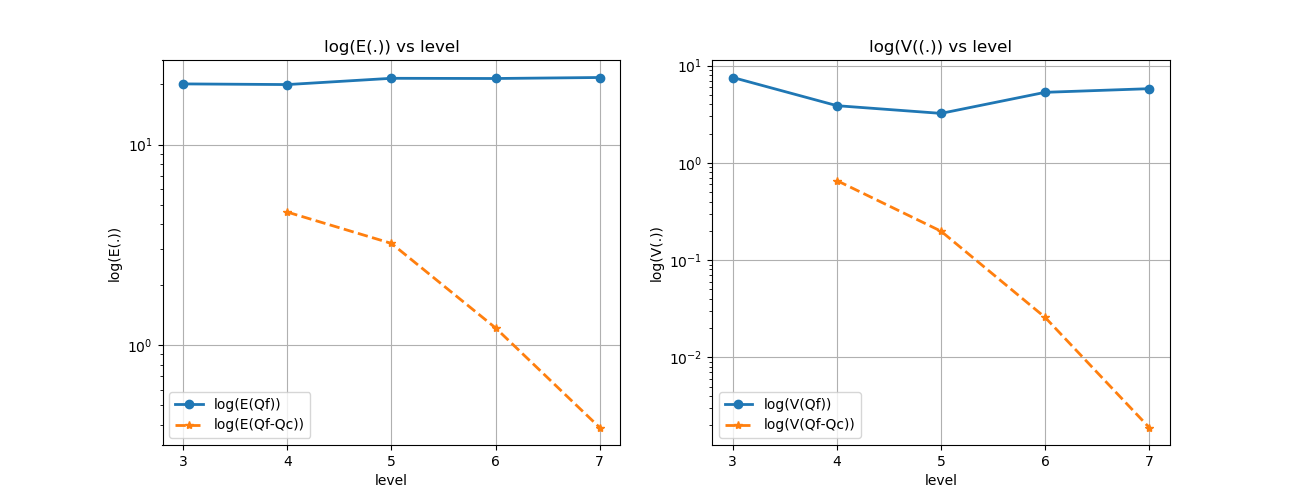
\includegraphics[width=0.49\textwidth]{../Aufgabe39/Sigma1lamda0.05/Figure_1.png}}	
	\subfigure[4.]{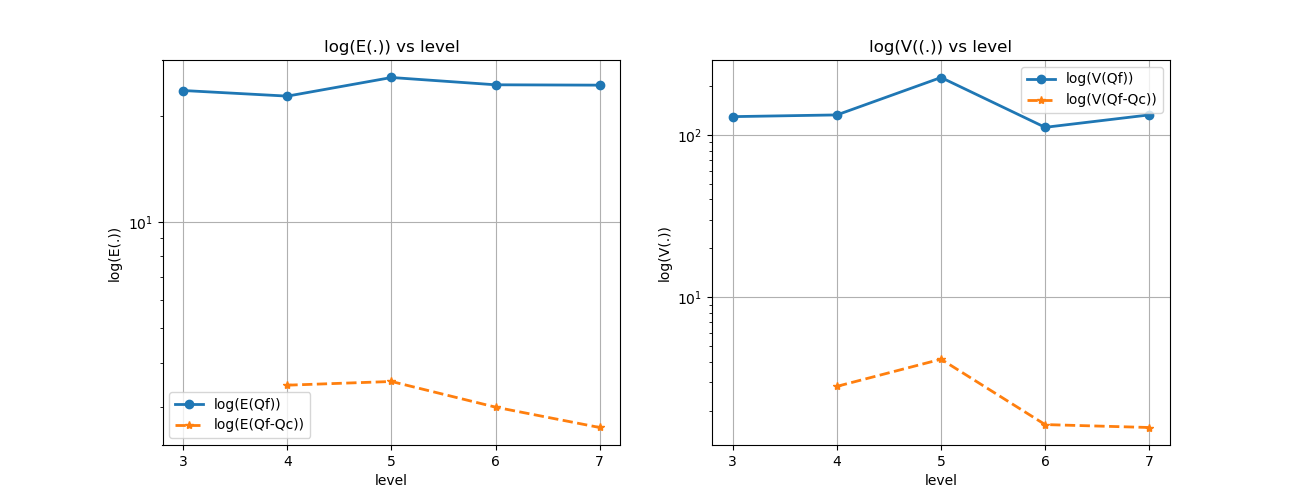
\includegraphics[width=0.49\textwidth]{../Aufgabe39/Sigma1alpha2.7/Figure_1.png}}	
\end{figure}

Anschließend testeten wir dann die MLMC-Methode für einer auf Konvergenz geprüfte Konfiguration, nämlich für $\sigma = 1$, $\lambda = 0.15$ und $\gamma = 2.7$
\begin{figure}[H]
	\centering
	\captionabove{MLMC Experiment für genannte Konfiguration}
	\subfigure{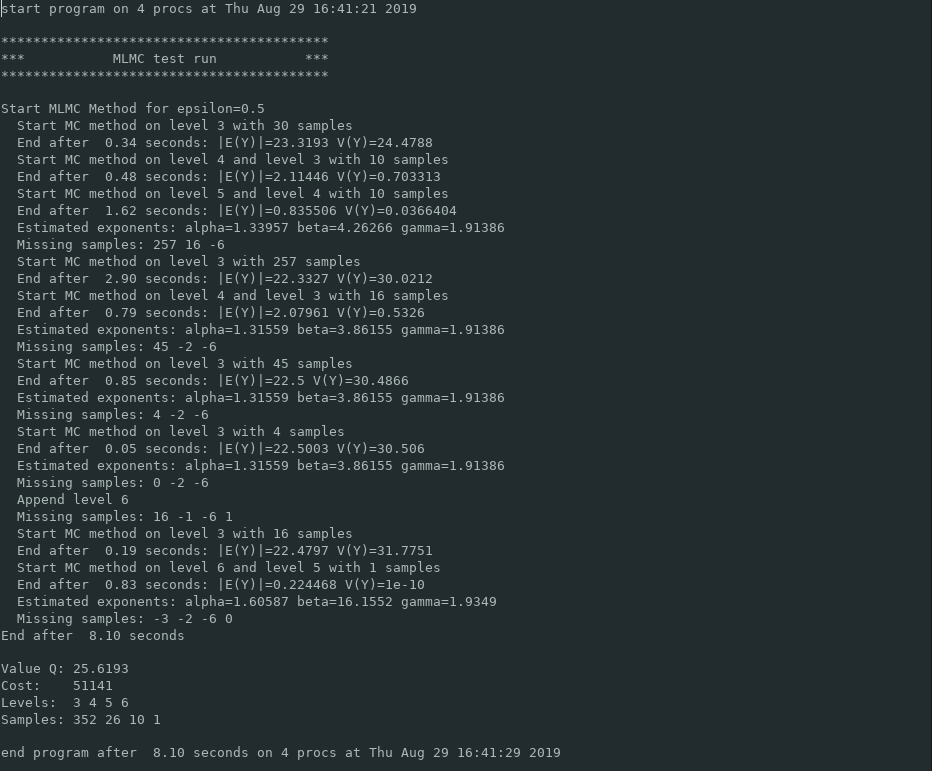
\includegraphics[width=0.89\textwidth]{../Aufgabe39/MLMCExp1/exp.png}}	 
\end{figure}

Man sieht sehr schön, dass der Algorithmus immer wieder einen MC-Ansatz auf einem bestimmten Level durchführt, dabei $| \mathbb{E}[Y] |$ und $\mathbb{V[Y]}$ berechnet und die Konvergenzparameter $\alpha , \beta, \gamma$ schätzt. Anschließend wird berechnet wie viele Samples auf den verschiedenen Leveln noch berechnet werden sollen. 
Erstaunlich ist dabei, dass wir auf dem höchsten Level tatsächlich nur ein einziges Sample berechnen müssen, um das gewünschte Level zu erreichen.
\begin{figure}[H]
	\centering
	\captionabove{Beispiel eines Samples mit Lösung (Streamlines) auf dem zweithöchsten Level}
	\subfigure{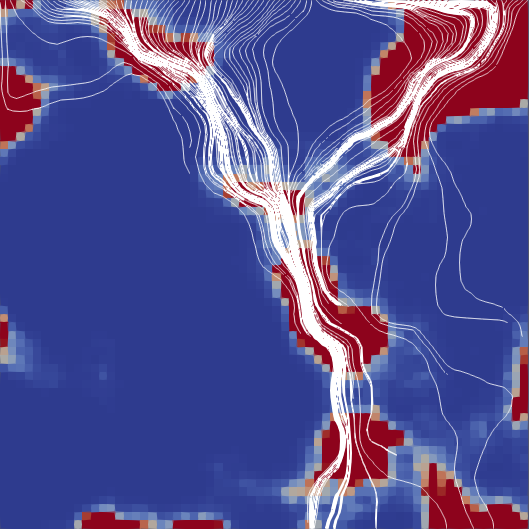
\includegraphics[width=0.49\textwidth]{../Aufgabe39/MLMCExp1/vtkshot.png}}	 
\end{figure}
Außerdem legt das Vorgehen des Algorithmus nahe ihn sozusagen 'adaptiv' zu nutzen. Statt also die initialen Sampleanzahlen $M_l$ festzulegen, legen wir verschiedene Fehler $\epsilon$ für die verschiedenen Level fest.
\begin{figure}[H]
	\centering
	\captionabove{MLMC Experiment über Epsilon}
	\subfigure{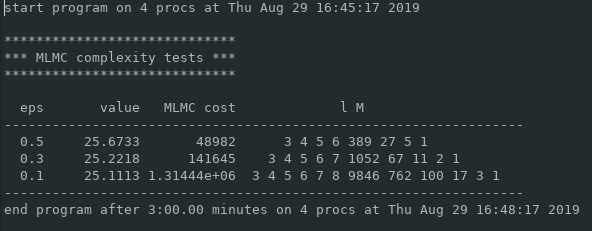
\includegraphics[width=0.99\textwidth]{../Aufgabe39/MLMCExpOverEps/exp2.png}}	 
\end{figure}
\begin{figure}[H]
	\centering
	\captionabove{Lösungsplot auf Level 8}
	\subfigure{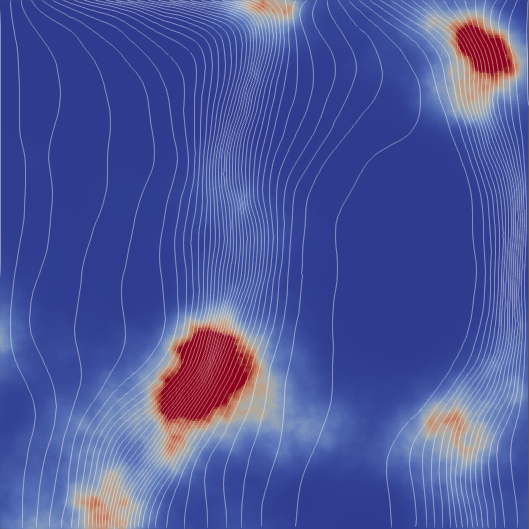
\includegraphics[width=0.49\textwidth]{../Aufgabe39/MLMCExpOverEps/res2.png}}	 
\end{figure}
Wir müssen also lediglich ein Sample auf Level 8 berechnen um unser vorgegebenes Epsilon zu erreichen.
Als Lösung (Spalte 'value') erhalten wir dabei den Erwartungswert des Zielfunktionals Q.

 





			
